\documentclass{article}
\usepackage{multicol}
\usepackage{graphicx}% Include figure files
\usepackage{dcolumn}% Align table columns on decimal point
\usepackage{bm}% bold math
\usepackage{hyperref}% add hypertext capabilities
\usepackage{booktabs}
\usepackage{listings}
\usepackage{mathtools}
\usepackage{amsmath}
\renewcommand{\abstractname}{\vspace{-\baselineskip}}
\bibliographystyle{plain}
\usepackage[utf8]{inputenc}
\usepackage{verbatim} %for å inkludere filer med tegn LaTeX ikke liker
\usepackage{mathpazo}
\usepackage{float}
\newcommand\numberthis{\addtocounter{equation}{1}\tag{\theequation}}

\begin{document}

\title{Project 3}
\author{Kandidatnummer}

\maketitle

\begin{abstract}

\end{abstract}

\begin{multicols}{2}

\section{Introduction}

Though simulating a solar system is interesting and fun enough on it's own, it is naturally also quite useful for the study of astrodynamics. In addition, being able to simulate a solar system provides a good set of tools applicable to many other scientific areas. These tools include having a good understanding of different numerical integration methods, and being able to write a structured and fast code. In this project we wish to explore a model of our own solar system, beginning with simulating the simple two-body system including the Earth and the Sun. We will use this system to compare two different methods of numerical integration, the forward Euler method and the velocity Verlet method. This simple system also makes a good testing ground for exploring whether our model is consistent with known physical laws such as energy conservation and Kepler's laws of planetary motion. We will also test the stability of the velocity Verlet method by including Jupiter and playing around with it's mass. From there we will include the rest of the planets in our solar system, and blah blah blag general relativity. 

\section{Theory}

The forward Euler method is an algorithm to estimate the solution of a differential equation. The Forward Euler method wants to find the next point $\mathbf{r}_{i+1}$. To find the next point, it uses the point it is at, $\mathbf{r}_{n}$, a small time step $dt$ and the derivative of its position. Which can be expressed as:

\begin{equation}
\mathbf{r}_{n+1}=\mathbf{r}_n + \mathbf{r}_n'\cdot dt
\label{eq:yn1}
\end{equation}


Where $y_{n+1}$ is the next step, $y_n$ is the current step, $y_n'$ is the derived of the current step and $dt$ is the time step.\\
This algorithm is really based abbreviated version of a Taylor expansion, where we only expand the series one step at a time. But by only taking one step at a time, we will also get a local truncation error, which causes an error for each step we take. 

\begin{equation}
\begin{split}
&y(t_n+dt)=y_{n+1}\\
&=y(t_n)+y_n'\cdot dt + R(dt^2)
\end{split}
\label{eq:ytndt}
\end{equation} 

Where $R(dt^2)$ is the local truncation error. Since the Forward Euler method is a first-order method, will the local truncation error be proportional to the square of the step size. 

\subsection{Velocity Verlet method}

The velocity Verlet method is based on the kinematic equations for an moving object, which in our case is the earth's orbit around the sun. If we want to find the next time step for the velocity and position we do a approximation and uses Taylor-expansion   

\begin{equation}
v_{t+dt}=v_t +\frac{dt}{2}(\frac{F_t}{m}+\frac{F_{t+m}}{m}) R(dt^3)
\label{eq:steps}
\end{equation}


We can also split the equation above and perform the calculation in several steps like this:

\begin{equation*}
\begin{split}
&v(t+\frac{1}{2}\Delta t)=v(t)+\frac{1}{2}a(t)\Delta t\\
&x(t+\Delta t)=x(t)+v(t+\frac{1}{2}\Delta t)\Delta t\\
&a(t+\Delta t)=f(x(t+\Delta t))\\
&v(t+\Delta t)=v(t+\frac{1}{2}\Delta t)+\frac{1}{2}a(t+\Delta t)\Delta t
\end{split}
\label{eq:steps}
\end{equation*}

\subsection{Conservation of angular momentum}
The definition of Keeplers law is that a area, where a connecting line between a planet and the sun, is always the same for an equal time interval. Which is illustrated in the figure below.

\begin{figure}[H]
	\centering
	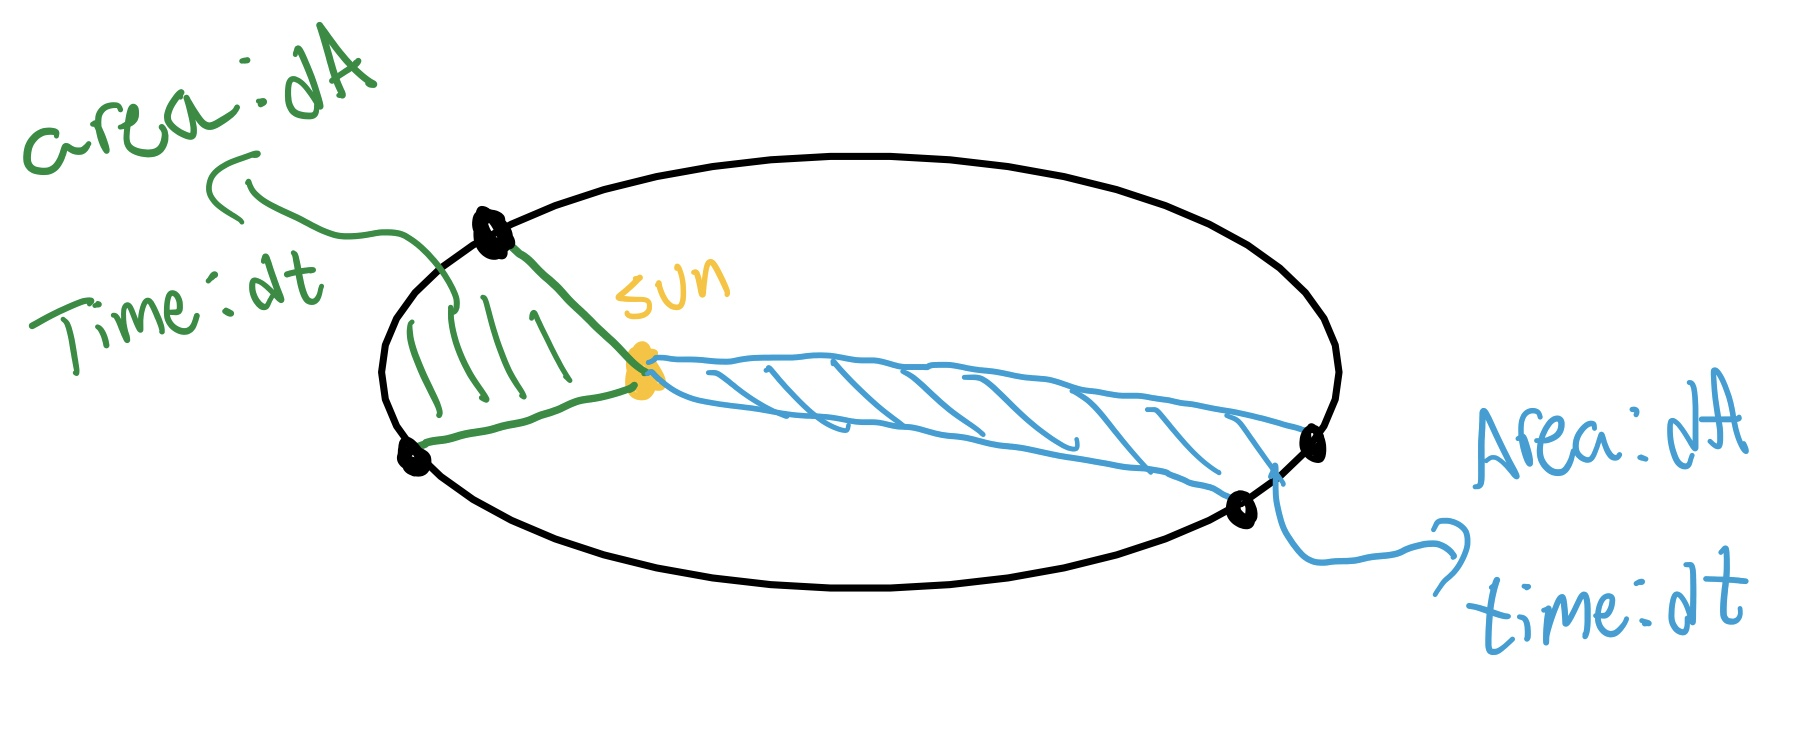
\includegraphics[width=\linewidth]{K2L.jpg}
	\caption{Keeplers second law. Where the area is the same for the same time interval.}
	\label{fig:1bplot}
\end{figure}

The best way to show that the angular momentum is conserved by using Keeplers second law is to make a drawing:

\begin{figure}[H]
	\centering
	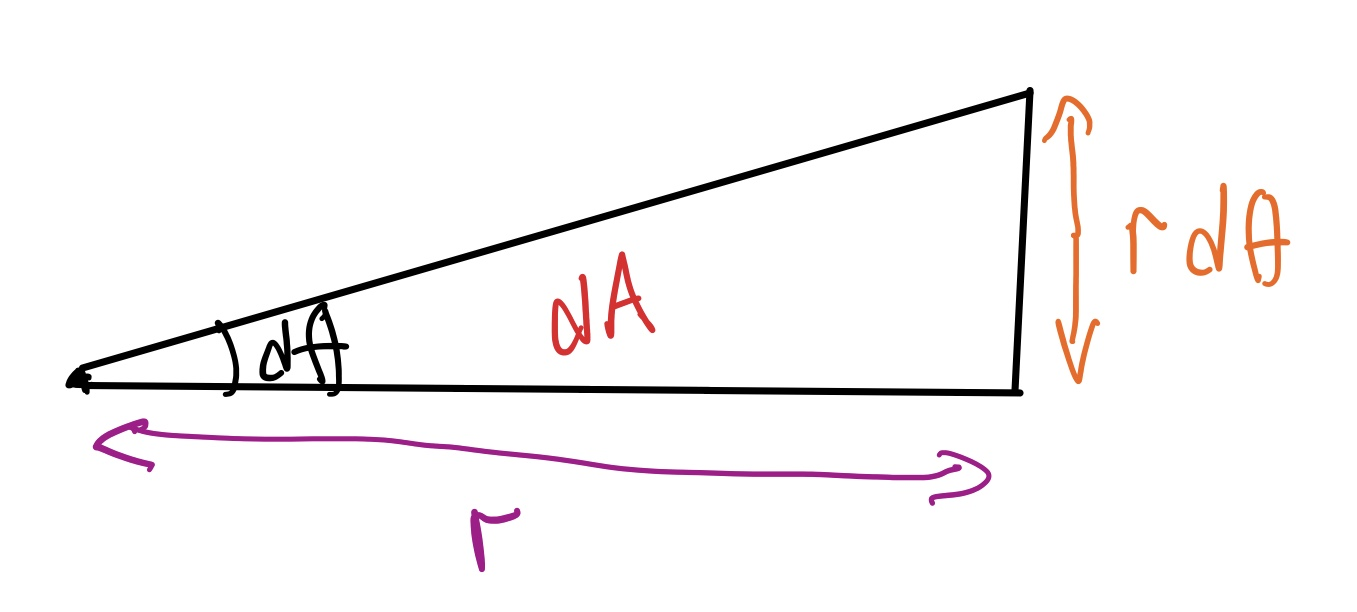
\includegraphics[width=\linewidth]{sketch.jpg}
	\caption{This square is the infinitesimal area dA that the planet has moved by a infinitesimal time interval dt}
	\label{fig:1bplot}
\end{figure}


Figure 2 shows us that the area is:

\begin{equation}
    dA=\frac{1}{2}r^2d\theta
\label{eq:dA}
\end{equation}

\end{multicols}

\clearpage

\appendix % Her kommer appendix.

\section{Calculations} 

\bibliography{References} % Kilder.
\begin{thebibliography}{9}
\bibitem{94}
	Skriv inn kilde her.
\end{thebibliography}

\end{document}
